% Options for packages loaded elsewhere
\PassOptionsToPackage{unicode}{hyperref}
\PassOptionsToPackage{hyphens}{url}
%
\documentclass[
]{book}
\usepackage{amsmath,amssymb}
\usepackage{lmodern}
\usepackage{iftex}
\ifPDFTeX
  \usepackage[T1]{fontenc}
  \usepackage[utf8]{inputenc}
  \usepackage{textcomp} % provide euro and other symbols
\else % if luatex or xetex
  \usepackage{unicode-math}
  \defaultfontfeatures{Scale=MatchLowercase}
  \defaultfontfeatures[\rmfamily]{Ligatures=TeX,Scale=1}
\fi
% Use upquote if available, for straight quotes in verbatim environments
\IfFileExists{upquote.sty}{\usepackage{upquote}}{}
\IfFileExists{microtype.sty}{% use microtype if available
  \usepackage[]{microtype}
  \UseMicrotypeSet[protrusion]{basicmath} % disable protrusion for tt fonts
}{}
\makeatletter
\@ifundefined{KOMAClassName}{% if non-KOMA class
  \IfFileExists{parskip.sty}{%
    \usepackage{parskip}
  }{% else
    \setlength{\parindent}{0pt}
    \setlength{\parskip}{6pt plus 2pt minus 1pt}}
}{% if KOMA class
  \KOMAoptions{parskip=half}}
\makeatother
\usepackage{xcolor}
\usepackage{longtable,booktabs,array}
\usepackage{calc} % for calculating minipage widths
% Correct order of tables after \paragraph or \subparagraph
\usepackage{etoolbox}
\makeatletter
\patchcmd\longtable{\par}{\if@noskipsec\mbox{}\fi\par}{}{}
\makeatother
% Allow footnotes in longtable head/foot
\IfFileExists{footnotehyper.sty}{\usepackage{footnotehyper}}{\usepackage{footnote}}
\makesavenoteenv{longtable}
\usepackage{graphicx}
\makeatletter
\def\maxwidth{\ifdim\Gin@nat@width>\linewidth\linewidth\else\Gin@nat@width\fi}
\def\maxheight{\ifdim\Gin@nat@height>\textheight\textheight\else\Gin@nat@height\fi}
\makeatother
% Scale images if necessary, so that they will not overflow the page
% margins by default, and it is still possible to overwrite the defaults
% using explicit options in \includegraphics[width, height, ...]{}
\setkeys{Gin}{width=\maxwidth,height=\maxheight,keepaspectratio}
% Set default figure placement to htbp
\makeatletter
\def\fps@figure{htbp}
\makeatother
\setlength{\emergencystretch}{3em} % prevent overfull lines
\providecommand{\tightlist}{%
  \setlength{\itemsep}{0pt}\setlength{\parskip}{0pt}}
\setcounter{secnumdepth}{5}
\usepackage{booktabs}
\ifLuaTeX
  \usepackage{selnolig}  % disable illegal ligatures
\fi
\usepackage[]{natbib}
\bibliographystyle{apalike}
\IfFileExists{bookmark.sty}{\usepackage{bookmark}}{\usepackage{hyperref}}
\IfFileExists{xurl.sty}{\usepackage{xurl}}{} % add URL line breaks if available
\urlstyle{same} % disable monospaced font for URLs
\hypersetup{
  pdftitle={Repositorio de oraciones para entrenamiento de guiones en español},
  pdfauthor={Yina Quique, PhD},
  hidelinks,
  pdfcreator={LaTeX via pandoc}}

\title{Repositorio de oraciones para entrenamiento de guiones en español}
\author{Yina Quique, PhD}
\date{2024-01-12}

\begin{document}
\maketitle

{
\setcounter{tocdepth}{1}
\tableofcontents
}
\hypertarget{intro}{%
\chapter*{Intro}\label{intro}}
\addcontentsline{toc}{chapter}{Intro}

\hypertarget{intro-en-espauxf1ol}{%
\section*{\texorpdfstring{Intro en \textbf{español}}{Intro en español}}\label{intro-en-espauxf1ol}}
\addcontentsline{toc}{section}{Intro en \textbf{español}}

Este repositorio se diseñó como parte de un proyecto financiado por el National Institute on Disability, Independent Living, and Rehabilitation Research (NIDILRR) Switzer Research Fellowship Program.

Usted encontrará un repositorio de oraciones diseñadas por hablantes de español con afasia, cuidadores, y clínicos trabajando con esta población. El repositorio es completamente \textbf{gratuito}.

Las oraciones pueden ser \textbf{usadas por personas con afasia que hablen español quienes quieran aprender oraciones de la vida cotidiana.} Las oraciones están diseñadas para ser aprendidas usando un software llamado Anki.

Necesitará un computador. También puede utilizar el repositorio desde su tablet o teléfono celular.

\hypertarget{intro-in-english}{%
\section*{\texorpdfstring{Intro in \textbf{English}}{Intro in English}}\label{intro-in-english}}
\addcontentsline{toc}{section}{Intro in \textbf{English}}

This repository was designed as part of a project funded by the National Institute on Disability, Independent Living, and Rehabilitation Research (NIDILRR) Switzer Research Fellowship Program.

You will find a sentence repository designed by Spanish speakers with aphasia, caregivers, and clinicians working with this population. The repository is completely \textbf{free}.

The sentences can be \textbf{used by Spanish-speaking people with aphasia who want to learn sentences to communicate in everyday situations.} The sentences are designed to be learned using software called Anki.

You will need a computer. You can also use the repository on your tablet or mobile phone.

\hypertarget{cross_0}{%
\chapter{Instrucciones para crear una cuenta en Anki y descargar el repositorio}\label{cross_0}}

\hypertarget{cree-una-cuenta-en-anki.}{%
\section{Cree una cuenta en Anki.}\label{cree-una-cuenta-en-anki.}}

En su computador, cree una cuenta de Anki. La cuenta se crea de forma \textbf{gratuita} en la siguiente página web.

\url{https://ankiweb.net/account/signup}

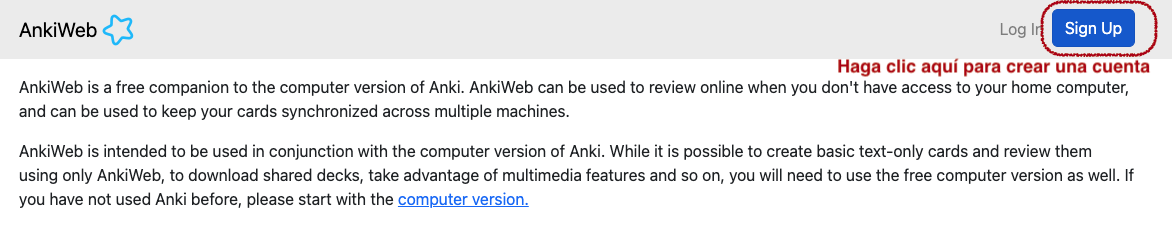
\includegraphics[width=0.9\linewidth]{images/reposit_sp/sign_up}

\hypertarget{cross_1}{%
\section{Escriba su email y cree una contraseña para Anki.}\label{cross_1}}

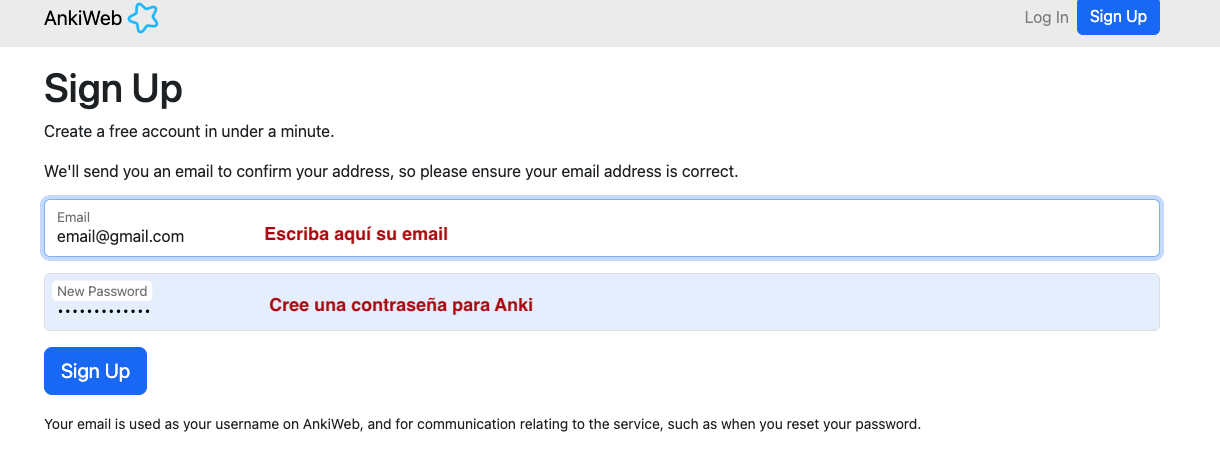
\includegraphics[width=0.9\linewidth]{images/reposit_sp/email_password}

\hypertarget{verifique-su-email.}{%
\section{Verifique su email.}\label{verifique-su-email.}}

Le llegará un correo electrónico a la cuenta de correo que usted indicó. \emph{Verifique} la cuenta dando clic en el enlace que le llegó a su correo.

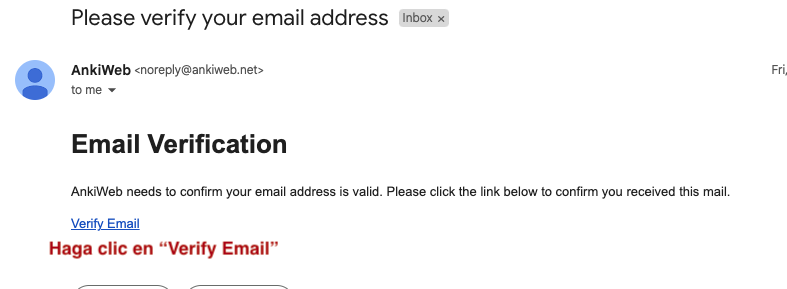
\includegraphics[width=0.9\linewidth]{images/reposit_sp/email_verification}

\hypertarget{descargue-anki-en-su-computador.}{%
\section{Descargue Anki en su computador.}\label{descargue-anki-en-su-computador.}}

Descargue Anki en su \emph{computador}, desde la siguiente página web:

\url{https://apps.ankiweb.net/}

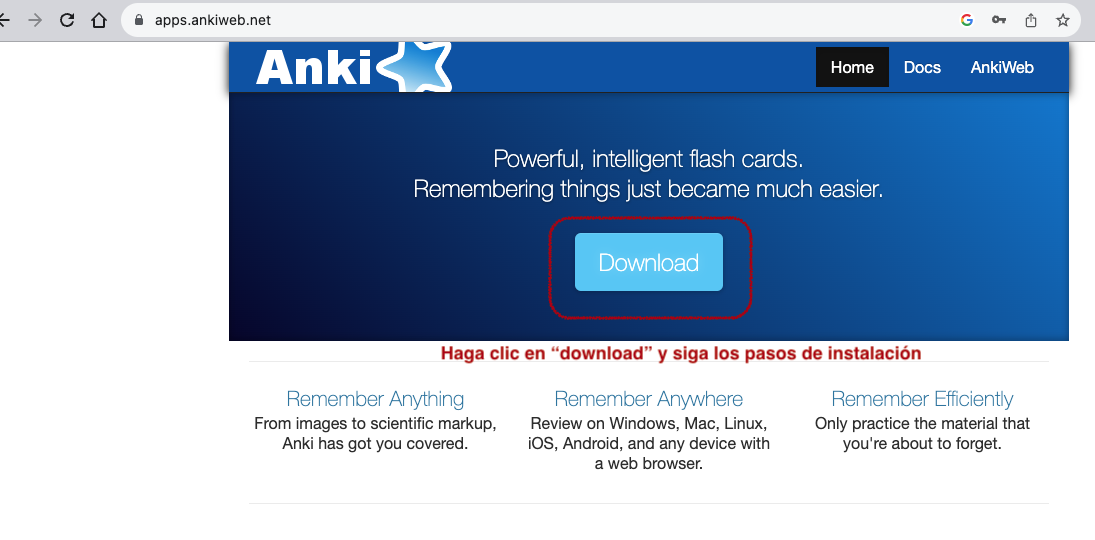
\includegraphics[width=0.6\linewidth]{images/reposit_sp/download}

\hypertarget{instale-anki-en-su-computador.}{%
\section{Instale Anki en su computador.}\label{instale-anki-en-su-computador.}}

Siga el proceso de instalación de Anki en su computador. Una vez terminada la instalación, Anki se verá \emph{similar} a la imagen que se muestra a continuación:

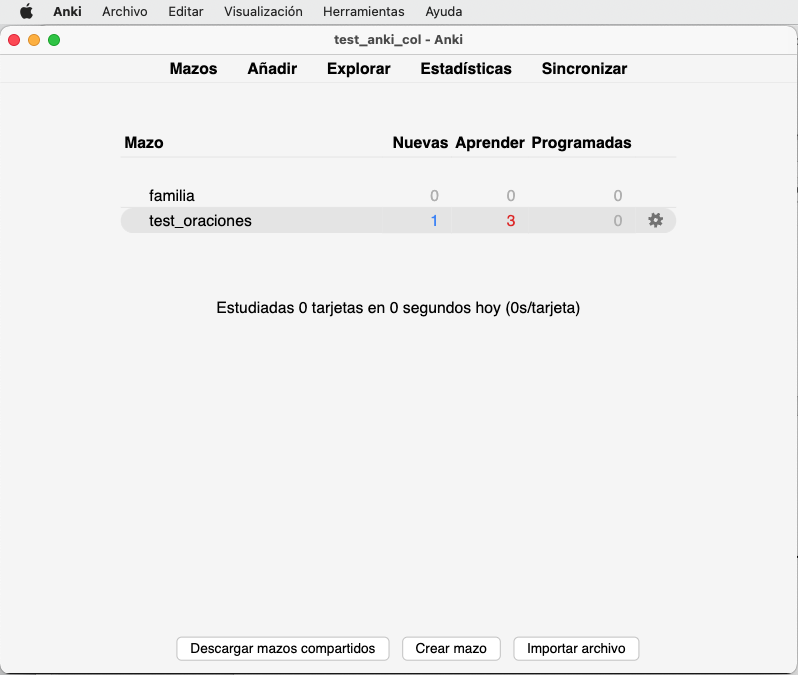
\includegraphics[width=0.6\linewidth]{images/reposit_sp/anki_screen}

\hypertarget{de-clic-en-sincronizar.}{%
\section{De clic en sincronizar.}\label{de-clic-en-sincronizar.}}


\includegraphics[width=0.6\linewidth]{images/reposit_sp/clic_sincronizar}

\hypertarget{ingrese-su-email-y-contraseuxf1a.-las-que-creuxf3-anteriormente-en-el-paso-1.2.}{%
\section{\texorpdfstring{Ingrese su email y contraseña. \protect\hyperlink{cross_1}{Las que creó anteriormente en el paso 1.2}.}{Ingrese su email y contraseña. Las que creó anteriormente en el paso 1.2.}}\label{ingrese-su-email-y-contraseuxf1a.-las-que-creuxf3-anteriormente-en-el-paso-1.2.}}

\hypertarget{descargue-el-repositorio.}{%
\section{Descargue el repositorio.}\label{descargue-el-repositorio.}}

\emph{Nota:} Intentamos hacer oraciones con género gramatical neutro, pero hay algunas que tienen marcadores de género (p.ej., estoy preocupad\textbf{a} vs.~Estoy preocupad\textbf{o}).

Existen dos archivos, uno con género gramatical femenino (fem.colpkg) y uno a género gramatical masculino (mas.colpkg). Por ejemplo, el archivo femenino tiene oraciones como \emph{estoy tranquila} y el masculino tiene oraciones como \emph{me siento solo.}

Aun así, las diferencias entre estos dos archivos son mínimas ya que la mayoría de las oraciones se comparten. \textbf{Seleccione el archivo con el que se identifique y descárguelo en su computador.}

Descargue el repositorio aquí descargue uno de los dos archivos, fem.colpkg o mas.colpkg:

\url{https://drive.google.com/drive/folders/1UgL4qijIzZTPCvqIir-spHCznOdJrdf8?usp=sharing}

\hypertarget{haga-doble-clic-en-el-archivo-que-descarguxf3.}{%
\section{Haga doble clic en el archivo que descargó.}\label{haga-doble-clic-en-el-archivo-que-descarguxf3.}}

Se va a demorar algunos minutos descargando y sincronizando. Tenga paciencia. Si da clic en \emph{sincronizar} verá algo parecido a la siguiente imagen.

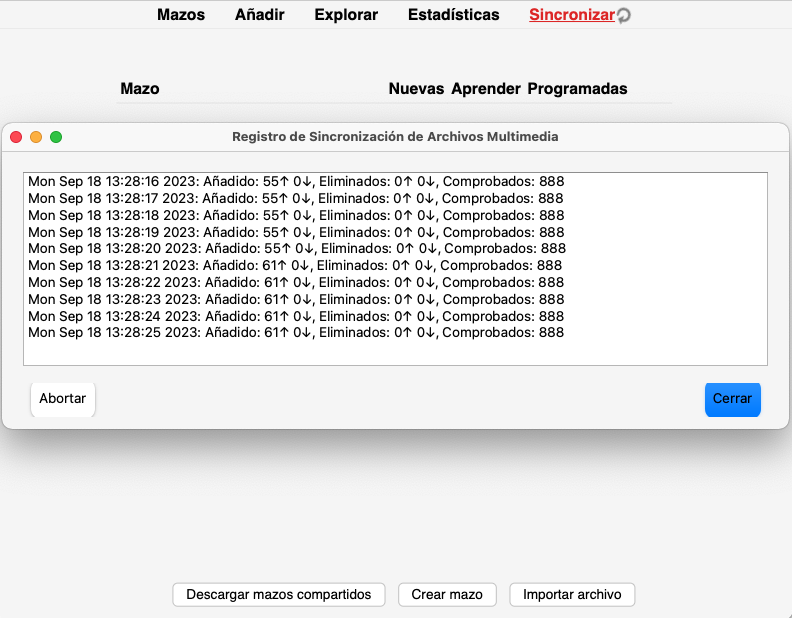
\includegraphics[width=0.6\linewidth]{images/reposit_sp/sincronizar}

\hypertarget{en-caso-de-que-le-salga-este-aviso-mientras-estuxe9-sincronizando-seleccione-la-opciuxf3n-subir-a-ankiweb.}{%
\section*{En caso de que le salga este aviso mientras esté sincronizando, seleccione la opción ``Subir a AnkiWeb.''}\label{en-caso-de-que-le-salga-este-aviso-mientras-estuxe9-sincronizando-seleccione-la-opciuxf3n-subir-a-ankiweb.}}
\addcontentsline{toc}{section}{En caso de que le salga este aviso mientras esté sincronizando, seleccione la opción ``Subir a AnkiWeb.''}

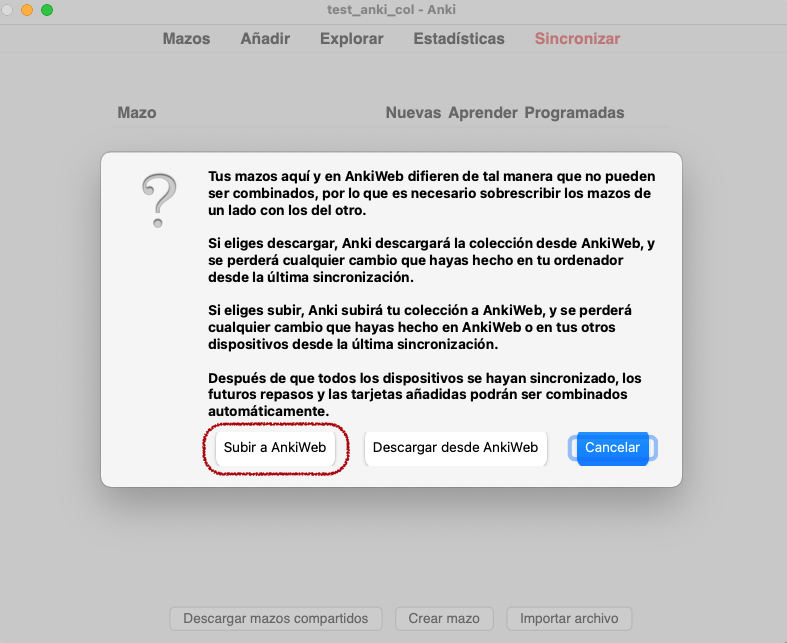
\includegraphics[width=0.6\linewidth]{images/reposit_sp/subir_a_anki}

\hypertarget{listo}{%
\section{¡Listo!}\label{listo}}

Una vez \emph{termine de sincronizar} el repositorio, estará listo para ser utilizado.

El siguiente paso es opcional y se trata de sincronizar el repositorio en su tablet o celular. Usted puede practicar en el computador, en la tablet, o en ambos.

Si no quiere o no necesita usar su tablet o celular para practicar, entonces pase a \protect\hyperlink{cross_4}{cómo practicar las oraciones.}

\hypertarget{instrucciones-para-usar-el-repositorio-en-su-tablet-o-celular}{%
\chapter{Instrucciones para usar el repositorio en su tablet o celular}\label{instrucciones-para-usar-el-repositorio-en-su-tablet-o-celular}}

Para seguir estos pasos debe haber \textbf{completado} las \protect\hyperlink{cross_0}{instrucciones para crear una cuenta en Anki y bajar el repositorio a su computador.}

\hypertarget{abra-su-app-store-si-tiene-un-iphone-o-play-store-si-tiene-un-android.}{%
\section{Abra su App store (si tiene un iPhone) o Play store (si tiene un Android).}\label{abra-su-app-store-si-tiene-un-iphone-o-play-store-si-tiene-un-android.}}

\hypertarget{busque-la-aplicaciuxf3n-llamada-anki.}{%
\section{Busque la aplicación llamada Anki.}\label{busque-la-aplicaciuxf3n-llamada-anki.}}

El \emph{ícono} de Anki se parece al siguiente:


\includegraphics[width=0.1\linewidth]{images/reposit_sp/Anki_logo}

\hypertarget{descargue-la-aplicaciuxf3n.}{%
\section{Descargue la aplicación.}\label{descargue-la-aplicaciuxf3n.}}

Descargue la aplicación en su tablet o celular. Tenga en cuenta que Anki es \textbf{gratis en Google play}, pero es de \textbf{pago en el App Store}.

\hypertarget{vincular-su-cuenta.}{%
\section{Vincular su cuenta.}\label{vincular-su-cuenta.}}

Entre a la aplicación de Anki y de clic en las \emph{tres líneas} que se encuentran generalmente en la parte izquierda de la pantalla

\includegraphics[width=0.3\linewidth]{images/reposit_sp/tres_lineas}

\hypertarget{seleccionar-estas-tres-luxedneas-abriruxe1-el-menuxfa-que-se-observa-a-continuaciuxf3n.}{%
\section{Seleccionar estas tres líneas abrirá el menú que se observa a continuación.}\label{seleccionar-estas-tres-luxedneas-abriruxe1-el-menuxfa-que-se-observa-a-continuaciuxf3n.}}

Seleccione en donde dice \emph{configuración}

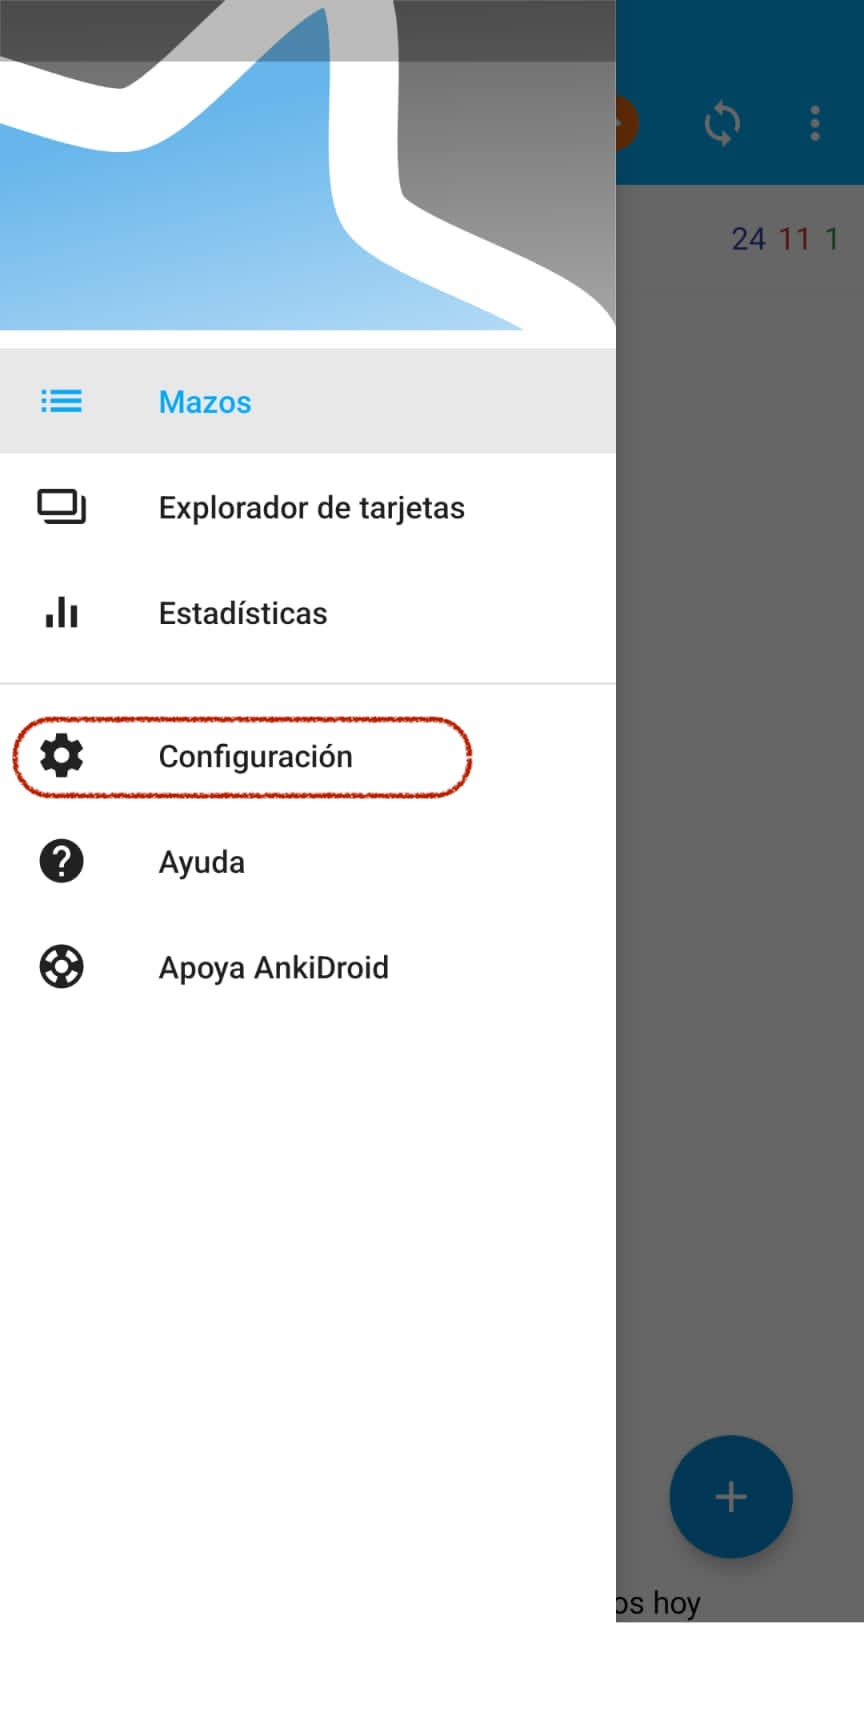
\includegraphics[width=0.3\linewidth]{images/reposit_sp/menu_config}

\hypertarget{ahora-seleccione-la-opciuxf3n-de-sincronizaciuxf3n}{%
\section{Ahora seleccione la opción de ``sincronización''}\label{ahora-seleccione-la-opciuxf3n-de-sincronizaciuxf3n}}

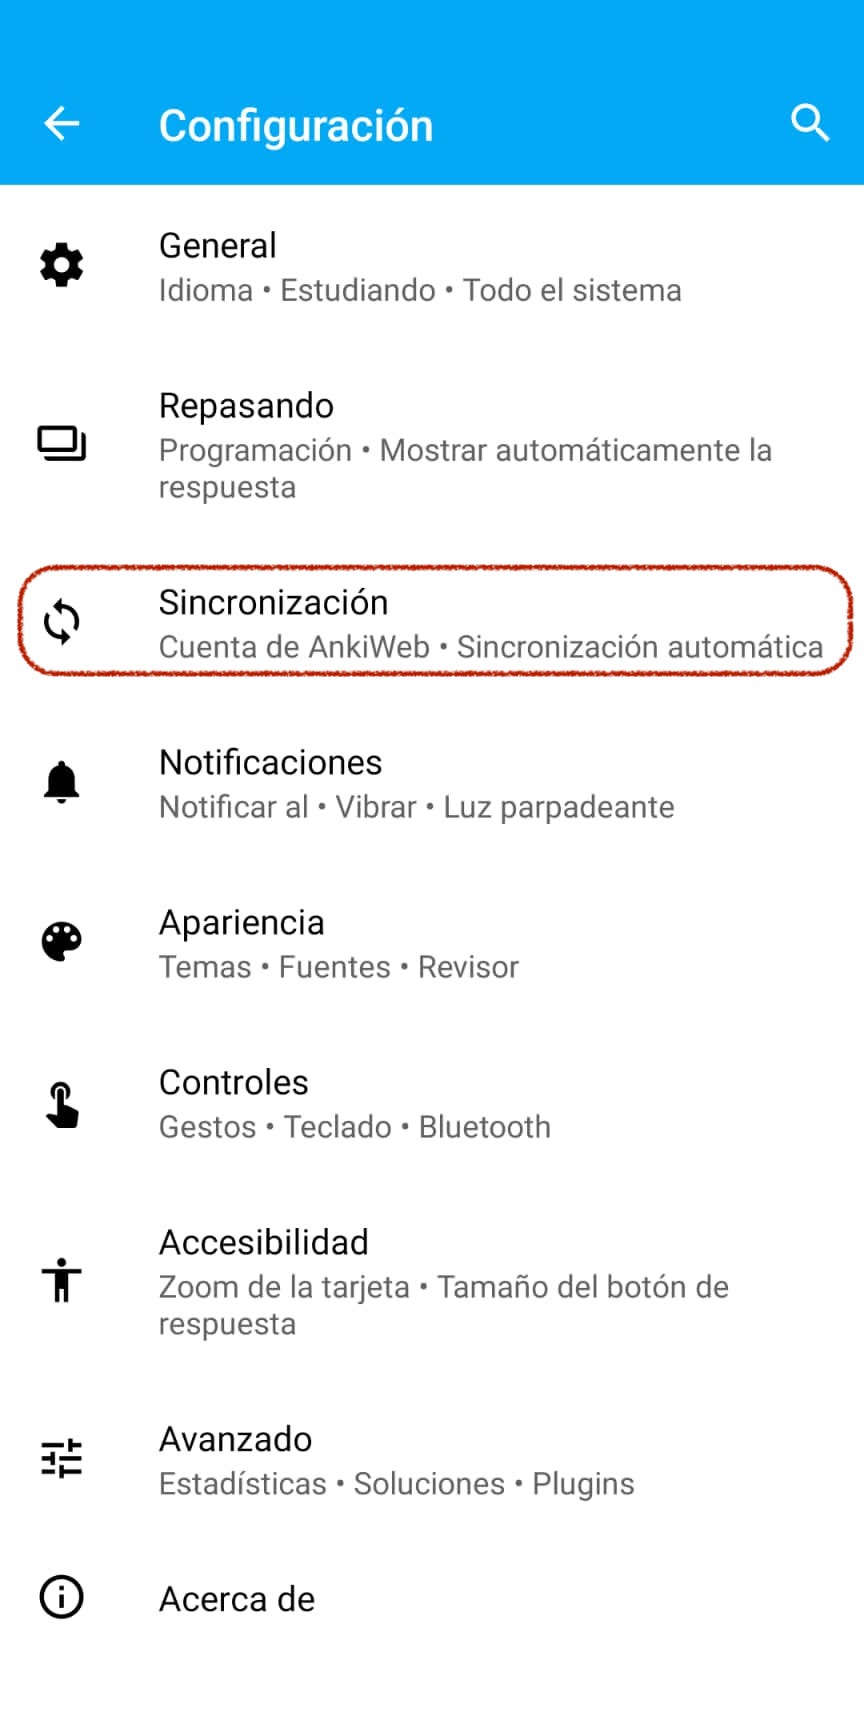
\includegraphics[width=0.3\linewidth]{images/reposit_sp/config_sincro}

\hypertarget{seleccione-la-opciuxf3n-cuenta-de-ankiweb.}{%
\section{Seleccione la opción ``Cuenta de AnkiWeb.''}\label{seleccione-la-opciuxf3n-cuenta-de-ankiweb.}}

Ponga su email y contraseña.\protect\hyperlink{cross_1}{El mismo email y contraseña que usó para crear la cuenta en Anki}

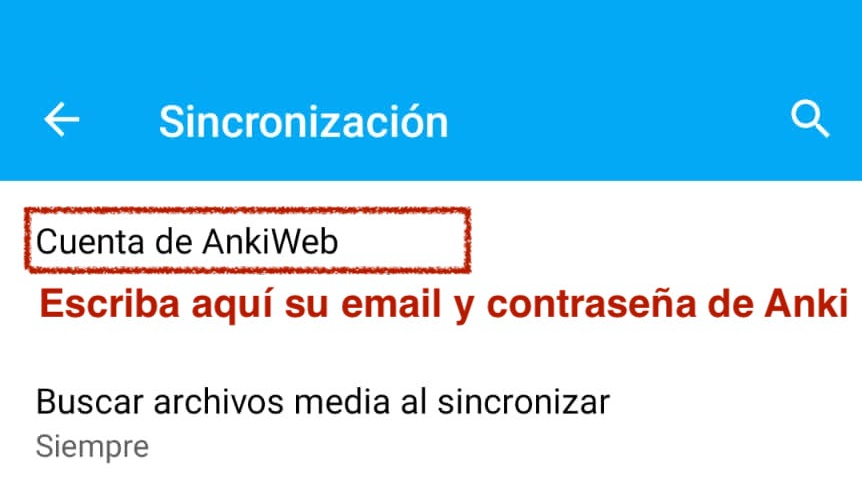
\includegraphics[width=0.3\linewidth]{images/reposit_sp/cuenta_anki1}

\textbf{Nota:} Puede ser también que deba ingresar su email y contraseña de Anki tan pronto abra la aplicación

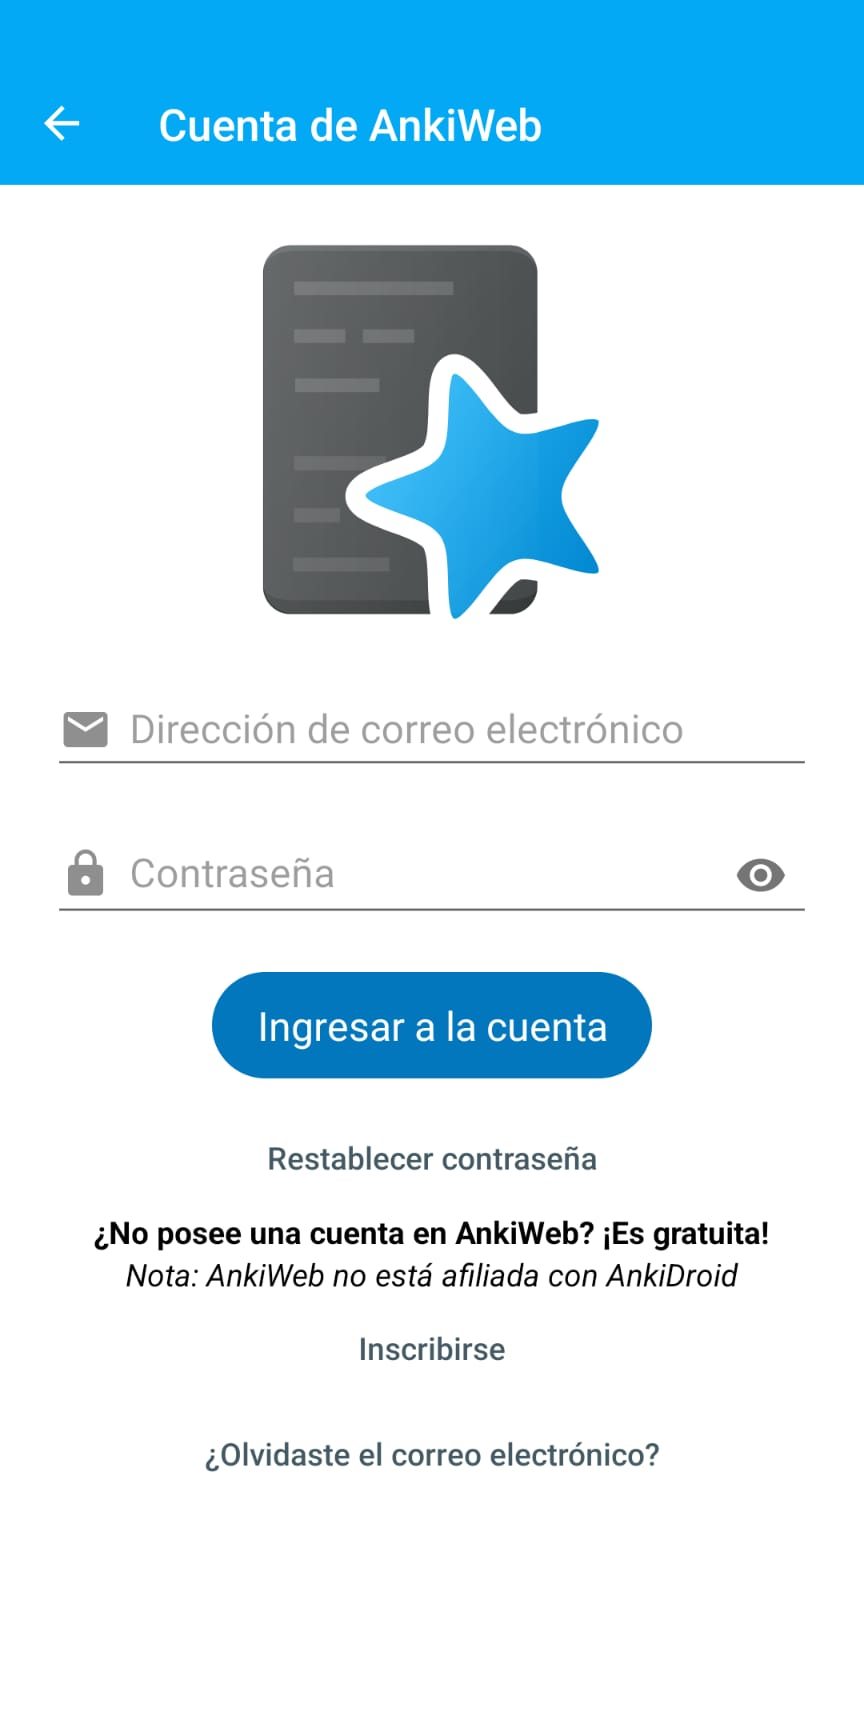
\includegraphics[width=0.3\linewidth]{images/reposit_sp/cuenta_anki2}

\hypertarget{se-tomaruxe1-unos-minutos-en-sincronizar-y-luego-veruxe1-el-repositorio.}{%
\section{Se tomará unos minutos en sincronizar y luego verá el repositorio.}\label{se-tomaruxe1-unos-minutos-en-sincronizar-y-luego-veruxe1-el-repositorio.}}

\hypertarget{cross_4}{%
\chapter{Pasos para estudiar oraciones}\label{cross_4}}

\emph{Nota:} En el siguiente video de apoyo se describen los pasos que deben seguir cada vez que vean una imagen/oración nueva.

\url{https://youtu.be/v-dNBT08lm0?si=_ehTlVFt6bwPHegl}

Además, en el siguiente link encontrarán los pasosde práctica para que los descarguen y los mantengan cerca de su computador/tablet/teléfono

\url{https://drive.google.com/file/d/17YQczy3QIZr6vow7PPEFlOrd2IbLUY2y/view?usp=drive_link}

Los pasos son los siguientes para aprender una oración nueva:

\hypertarget{cross_2}{%
\section{Escucha}\label{cross_2}}

\emph{Escuchen} la oración dando clic o tocando el ícono 
\includegraphics{images/play_icon.png} Escuchen SIN hablar.

\hypertarget{escucha-y-seuxf1ala}{%
\section{Escucha y señala}\label{escucha-y-seuxf1ala}}

Escuchen nuevamente la oración dando clic o tocando el ícono 
\includegraphics{images/play_icon.png} \emph{Mientras escuchan, señalen} con su dedo palabra por palabra de la oración escrita.

\hypertarget{juntos}{%
\section{Juntos}\label{juntos}}

Intenten decir la oración \emph{al mismo tiempo} que el video. Hagan este paso \textbf{dos} veces. Para esto, nuevamente necesitarán dar clic o tocar el ícono 
\includegraphics{images/play_icon.png}

\hypertarget{tuxfa-solo}{%
\section{Tú solo}\label{tuxfa-solo}}

Intenten decir la oración \emph{sin} ayuda del video.

\hypertarget{califica}{%
\section{Califica}\label{califica}}

Califiquen su producción usando las \emph{siguientes opciones}:

\begin{itemize}
\item
  Otra vez = ``no lo logré hacer muy bien y necesito hacerlo otra vez.''
\item
  Difícil = ``lo hice más o menos''
\item
  Bien = ``lo hice bien''
\item
  Fácil = Ignoren esta opción por ahora
\end{itemize}

\hypertarget{importante-si-es-una-oraciuxf3n-que-ya-han-visto-antes-del-paso-1-intente-recordar-la-oraciuxf3n-con-ayuda-de-la-imagen.}{%
\section{\texorpdfstring{¡Importante! Si es una oración que \textbf{ya} han visto, ANTES del \protect\hyperlink{cross_2}{paso 1}, intente recordar la oración con ayuda de la imagen.}{¡Importante! Si es una oración que ya han visto, ANTES del paso 1, intente recordar la oración con ayuda de la imagen.}}\label{importante-si-es-una-oraciuxf3n-que-ya-han-visto-antes-del-paso-1-intente-recordar-la-oraciuxf3n-con-ayuda-de-la-imagen.}}

\hypertarget{los-pasos-descritos-aquuxed-son-basados-en-la-evidencia-cientuxedfica-de-un-tratamiento-llamado-script-training.}{%
\section{\texorpdfstring{Los pasos descritos aquí son \emph{basados en la evidencia científica} de un tratamiento llamado Script Training.}{Los pasos descritos aquí son basados en la evidencia científica de un tratamiento llamado Script Training.}}\label{los-pasos-descritos-aquuxed-son-basados-en-la-evidencia-cientuxedfica-de-un-tratamiento-llamado-script-training.}}

\hypertarget{cross_3}{%
\chapter{Instructions to create an Anki account and download the repository}\label{cross_3}}

\hypertarget{create-an-account-on-anki.}{%
\section{Create an account on Anki.}\label{create-an-account-on-anki.}}

Using your computer, start by creating an Anki account. Creating an account is \textbf{free}. Visit the following website to do so:

\url{https://ankiweb.net/account/signup}

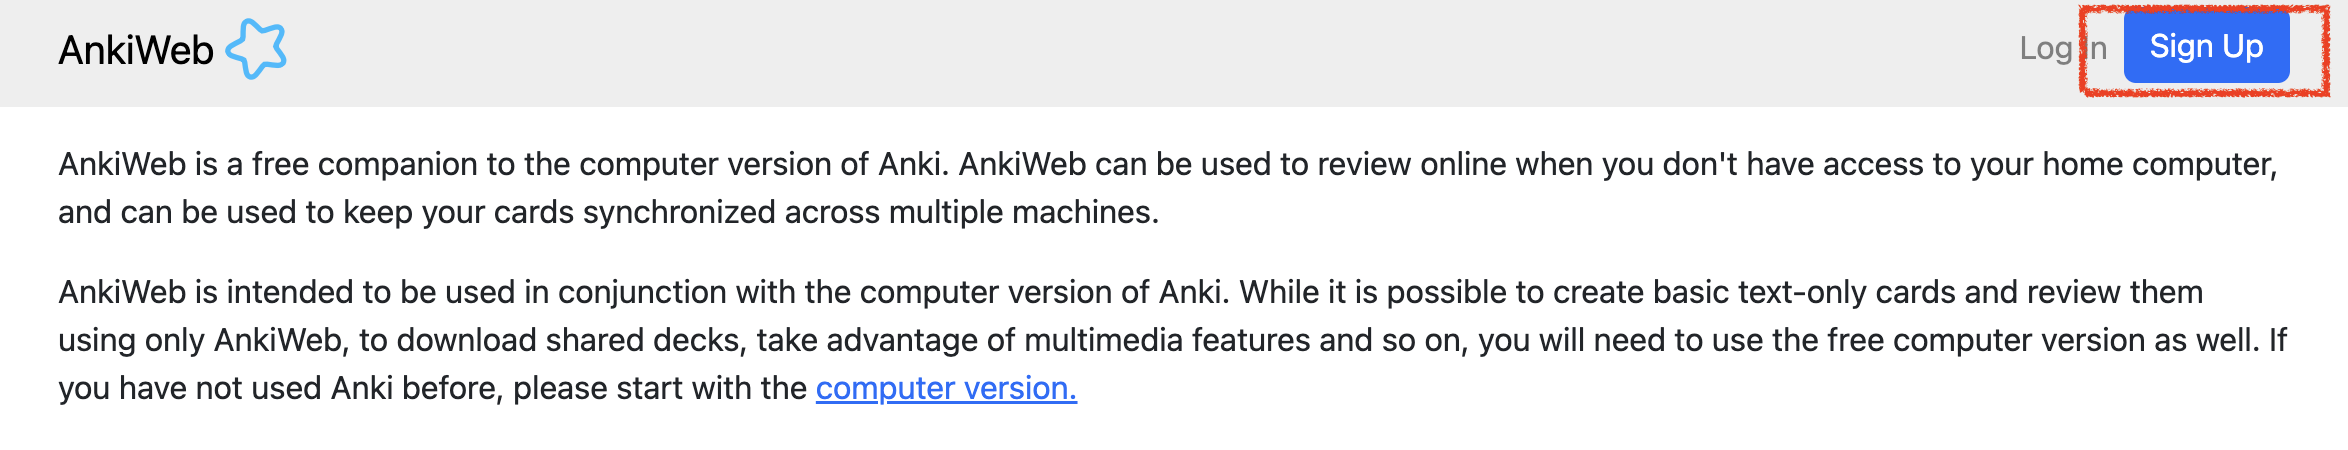
\includegraphics[width=0.9\linewidth]{images/reposit_en/sign_up}

\hypertarget{cross_3}{%
\section{Enter your email and create a password for Anki.}\label{cross_3}}

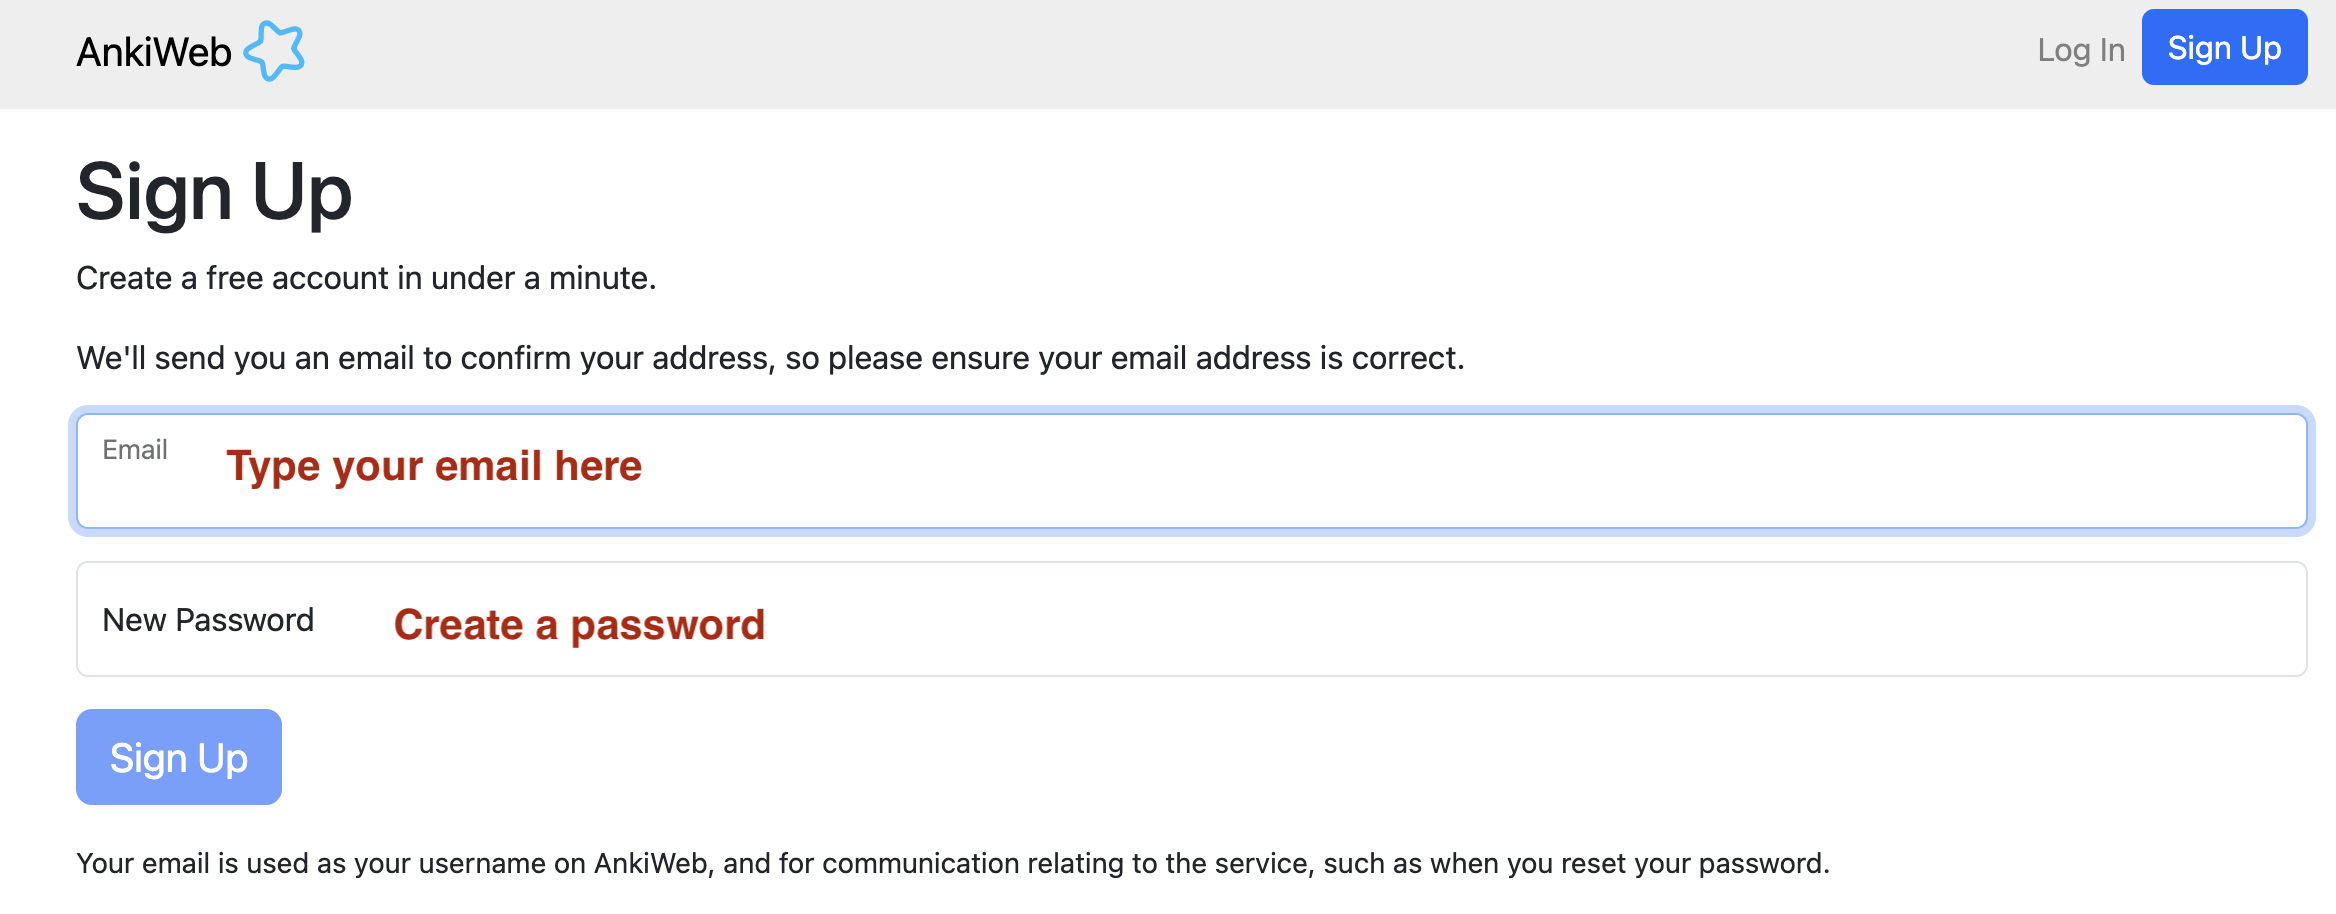
\includegraphics[width=0.9\linewidth]{images/reposit_en/email_password}

\hypertarget{check-your-email.}{%
\section{Check your email.}\label{check-your-email.}}

An email will be sent to the email account you indicated. \emph{Verify} the account by clicking on the link sent to your email.

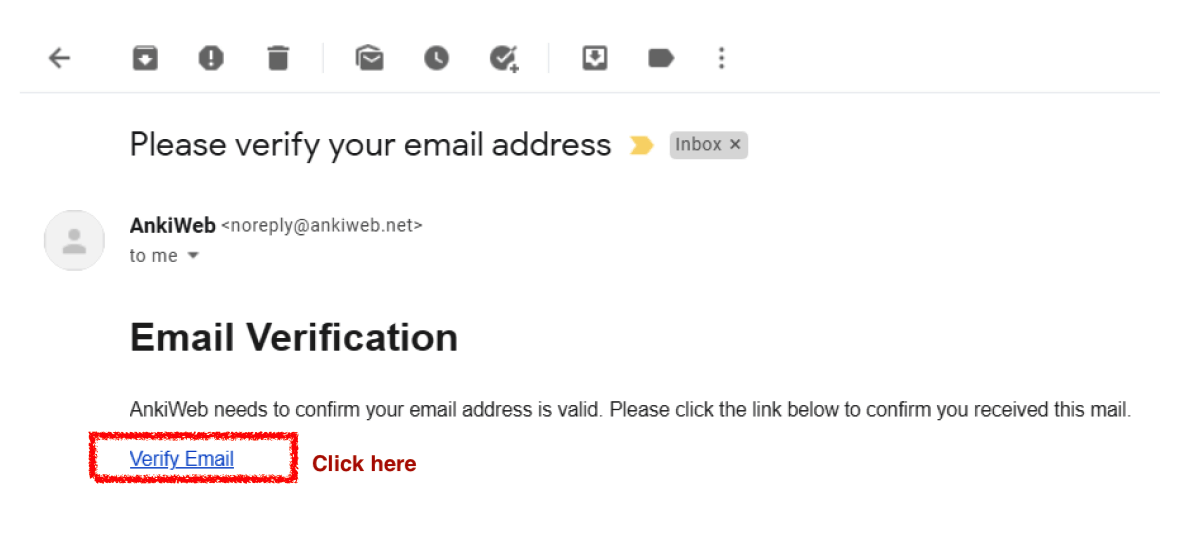
\includegraphics[width=0.9\linewidth]{images/reposit_en/email_verification}

\hypertarget{download-anki-to-your-computer.}{%
\section{Download Anki to your computer.}\label{download-anki-to-your-computer.}}

Download Anki to your \textbf{computer} from this website:

\url{https://apps.ankiweb.net/}

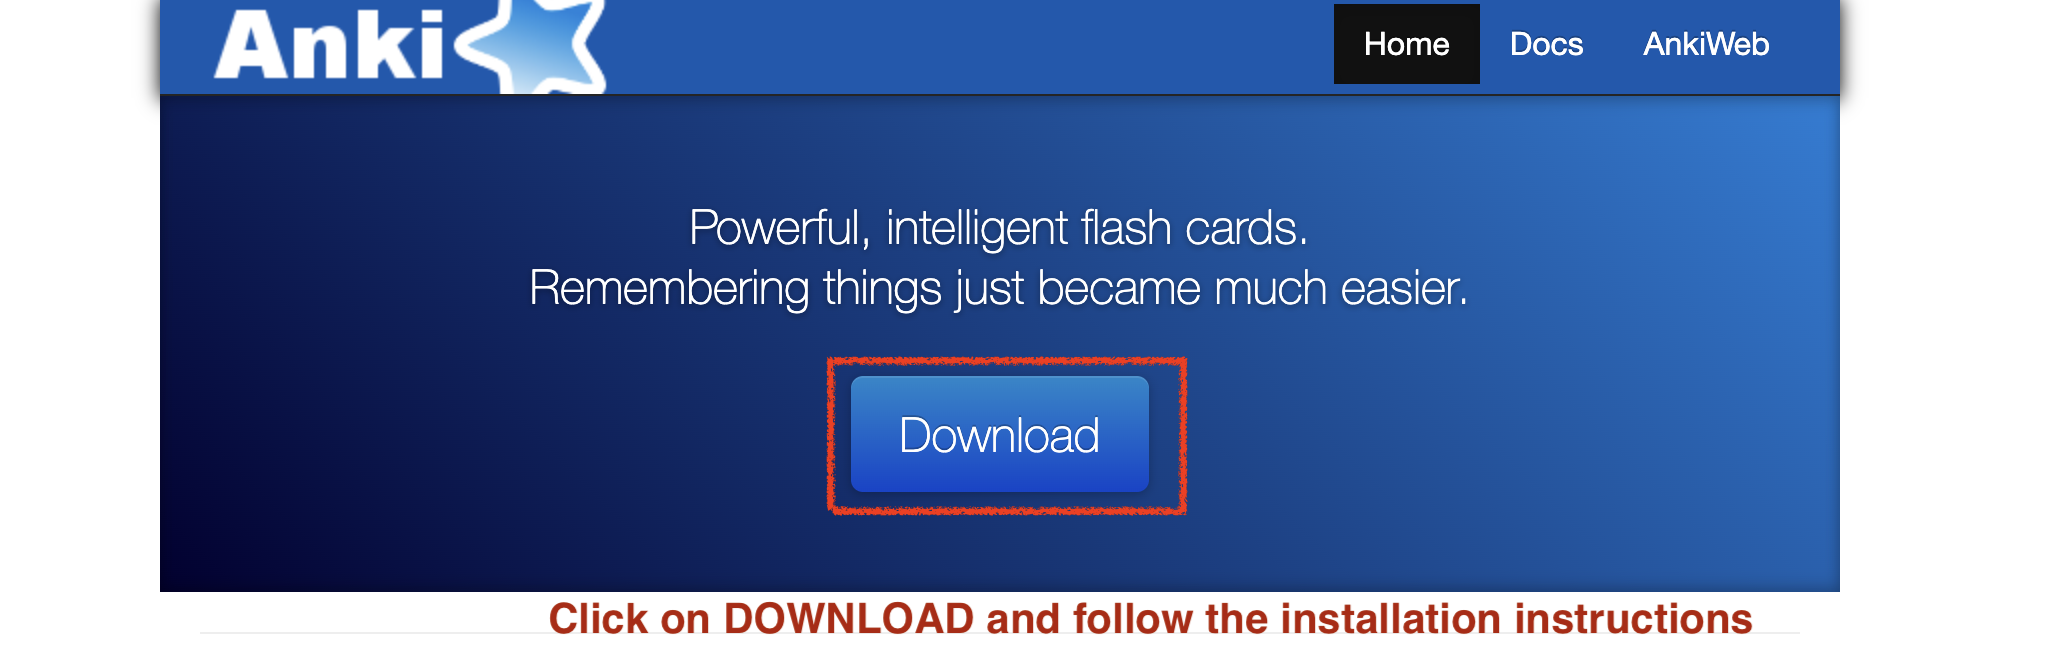
\includegraphics[width=0.6\linewidth]{images/reposit_en/download}

\hypertarget{install-anki-on-your-computer.}{%
\section{Install Anki on your computer.}\label{install-anki-on-your-computer.}}

Follow the Anki installation process on your computer. Once the installation is complete, Anki will look \emph{similar} to the image below:

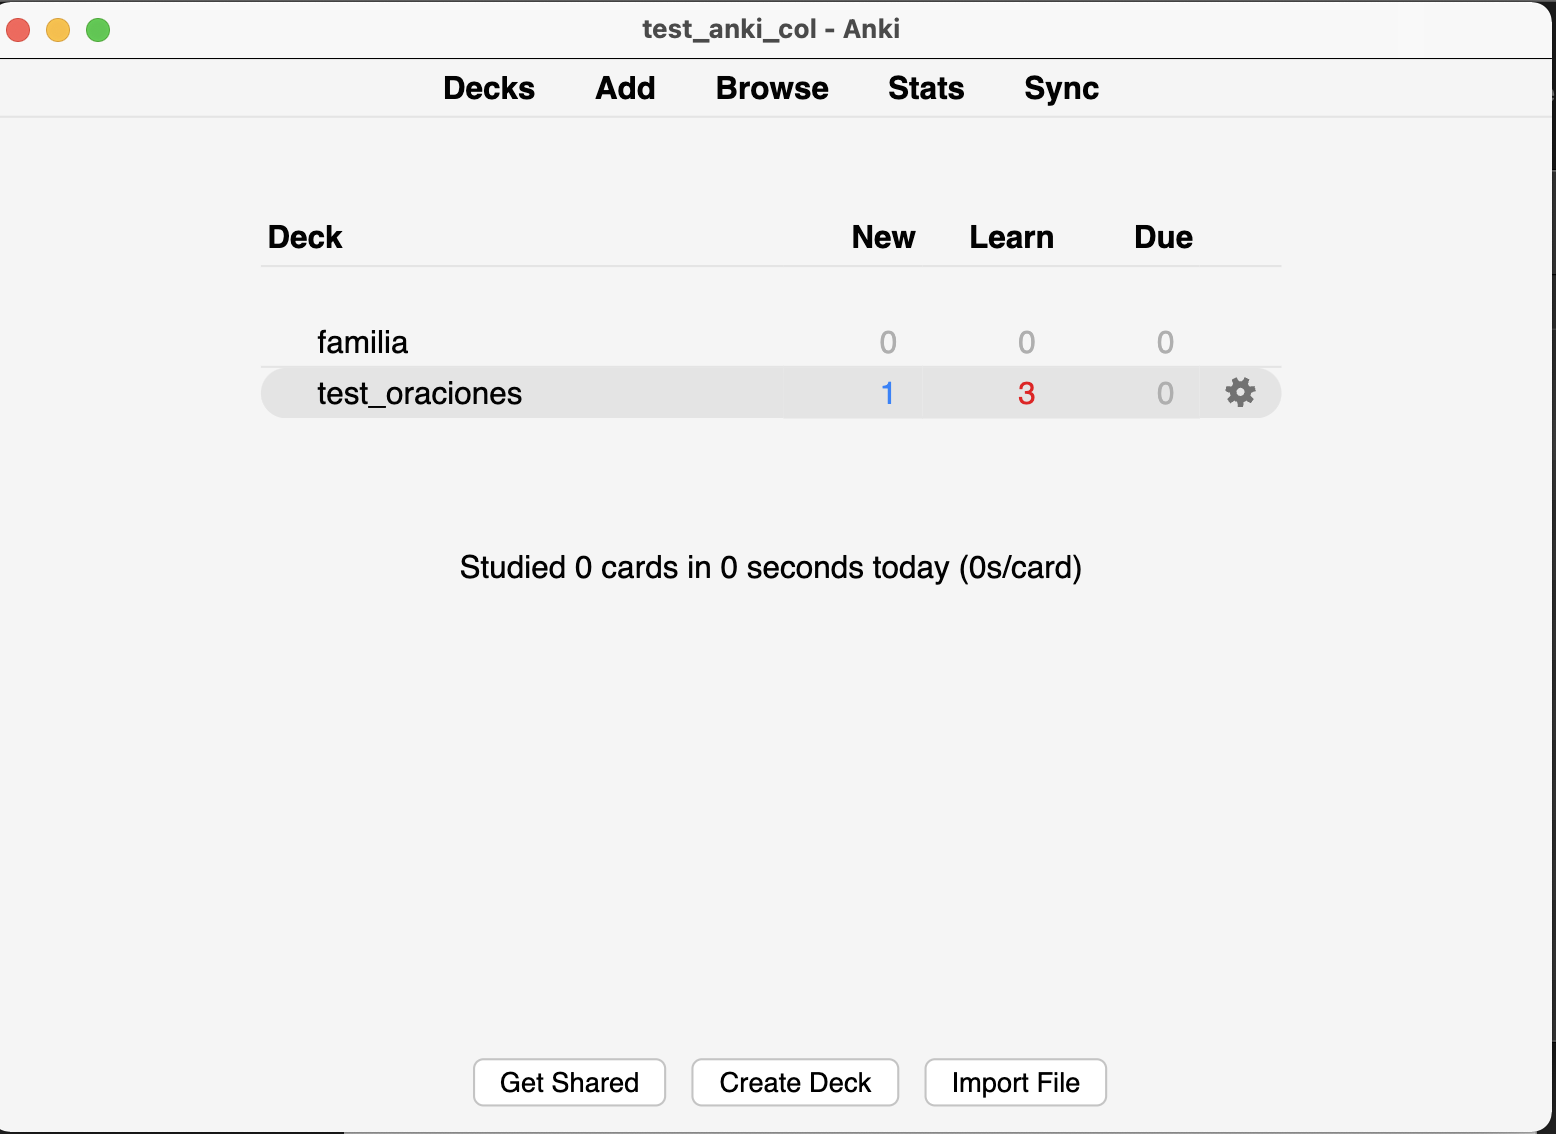
\includegraphics[width=0.6\linewidth]{images/reposit_en/anki_screen}

\hypertarget{click-on-sync.}{%
\section{Click on sync.}\label{click-on-sync.}}

\hypertarget{enter-your-email-and-password.-the-ones-you-created-previously-in-4.2.}{%
\section{\texorpdfstring{Enter your email and password. \protect\hyperlink{cross_3}{The ones you created previously in 4.2}.}{Enter your email and password. The ones you created previously in 4.2.}}\label{enter-your-email-and-password.-the-ones-you-created-previously-in-4.2.}}

\hypertarget{download-the-repository.}{%
\section{Download the repository.}\label{download-the-repository.}}

\emph{Note:} We tried to make gender-neutral sentences in Spanish (grammatically speaking), but some sentences have grammatical gender markers (e.g., estoy preocupad\textbf{a} vs.~Estoy preocupad\textbf{o}).

There are two files: one with feminine gender markers (fem.colpkg) and one with masculine gender markers (mas.colpkg). For example, the feminine file has sentences like \emph{estoy tranquila} and the masculine file has sentences like \emph{me siento solo.}

Still, the differences between these two files are minimal since most of the sentences are shared. \textbf{Select the file with which you identify yourself and download it to your computer.}

Download the repository here (download either fem.colpkg or mas.colpkg) \url{https://drive.google.com/drive/folders/1UgL4qijIzZTPCvqIir-spHCznOdJrdf8?usp=sharing}

\hypertarget{double-click-the-file-you-downloaded.}{%
\section{Double click the file you downloaded.}\label{double-click-the-file-you-downloaded.}}

It will take a few minutes to download and synchronize. Have patience.

\hypertarget{if-you-see-this-prompt-while-synchronizing-select-the-upload-to-ankiweb-option.}{%
\section*{If you see this prompt while synchronizing, select the ``Upload to AnkiWeb'' option.}\label{if-you-see-this-prompt-while-synchronizing-select-the-upload-to-ankiweb-option.}}
\addcontentsline{toc}{section}{If you see this prompt while synchronizing, select the ``Upload to AnkiWeb'' option.}

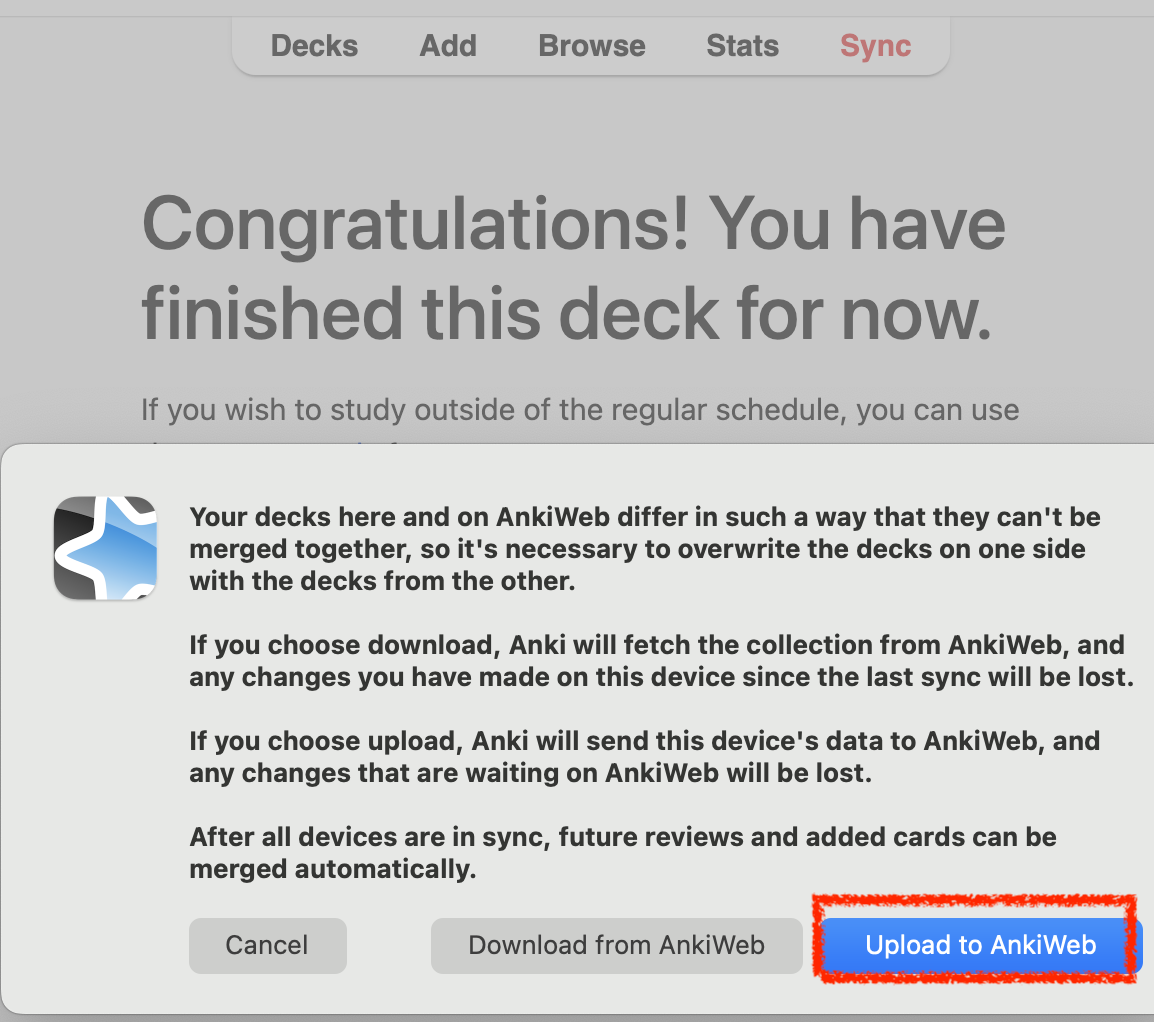
\includegraphics[width=0.6\linewidth]{images/reposit_en/subir_a_anki}

\hypertarget{you-are-ready}{%
\section{You are ready!}\label{you-are-ready}}

Once it \emph{finishes synchronizing,} the repository will be ready to be used.

The next step is optional and involves synchronizing the repository on your tablet or phone. You can practice on the computer, tablet, or both.

If you don't want or need to use your tablet or phone to practice, then skip to \protect\hyperlink{cross_5}{how to practice sentences.}

\hypertarget{instructions-to-use-the-repository-on-your-tablet-or-phone}{%
\chapter{Instructions to use the repository on your tablet or phone}\label{instructions-to-use-the-repository-on-your-tablet-or-phone}}

To follow these steps you must have \textbf{completed} the \protect\hyperlink{cross_3}{instructions to create an Anki account and download the repository to your computer.}

\hypertarget{open-your-app-store-if-you-have-an-iphone-or-play-store-if-you-have-an-android.}{%
\section{Open your App store (if you have an iPhone) or Play store (if you have an Android).}\label{open-your-app-store-if-you-have-an-iphone-or-play-store-if-you-have-an-android.}}

\hypertarget{look-for-the-app-called-anki.}{%
\section{Look for the app called Anki.}\label{look-for-the-app-called-anki.}}

The Anki \emph{icon} looks like this:


\includegraphics[width=0.1\linewidth]{images/reposit_en/Anki_logo}

\hypertarget{download-the-app.}{%
\section{Download the app.}\label{download-the-app.}}

Download the app on your tablet or phone. Please note that Anki is \textbf{free on Google play}, but requires \textbf{payment on the App Store.}

\hypertarget{link-your-account.}{%
\section{Link your account.}\label{link-your-account.}}

Enter the app and click on the \textbf{three lines} usually found on the left side of the screen.

\includegraphics[width=0.3\linewidth]{images/reposit_en/tres_lineas}

\hypertarget{selecting-these-three-lines-will-open-the-menu-seen-below.}{%
\section{Selecting these three lines will open the menu seen below.}\label{selecting-these-three-lines-will-open-the-menu-seen-below.}}

Select where it says \emph{settings}

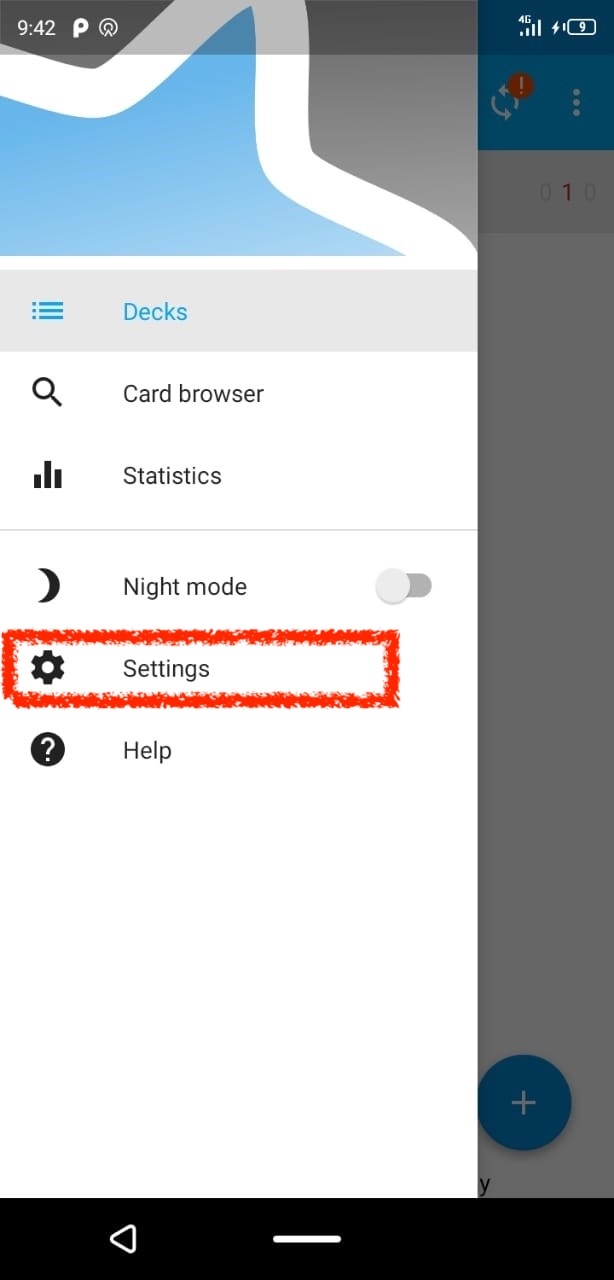
\includegraphics[width=0.3\linewidth]{images/reposit_en/menu_config}

\hypertarget{now-select-the-sync-option}{%
\section{Now select the ``sync'' option}\label{now-select-the-sync-option}}

\hypertarget{select-the-ankiweb-account-option.}{%
\section{Select the ``AnkiWeb Account'' option.}\label{select-the-ankiweb-account-option.}}

Enter your email and password.\protect\hyperlink{cross_3}{The same email and password you used to create the Anki account}

\textbf{Note:} You may also be required to enter your Anki email and password as soon as you open the app.

\hypertarget{it-will-take-a-few-minutes-to-sync-and-then-you-will-see-the-repository.}{%
\section{It will take a few minutes to sync and then you will see the repository.}\label{it-will-take-a-few-minutes-to-sync-and-then-you-will-see-the-repository.}}

\hypertarget{cross_5}{%
\chapter{Steps to study sentences}\label{cross_5}}

\emph{Note:} This support video describes the steps to follow when seeing a new image/sentence.

\url{https://youtu.be/v-dNBT08lm0?si=_ehTlVFt6bwPHegl}

Additionally, in the link below, you will find the practice steps to keep them close to your computer/tablet/phone

\url{https://drive.google.com/file/d/17YQczy3QIZr6vow7PPEFlOrd2IbLUY2y/view?usp=drive_link}

The steps are as follows to learn a new sentence:

\hypertarget{cross_6}{%
\section{Listen}\label{cross_6}}

\emph{Listen} to the sentence by clicking icon 
\includegraphics{images/play_icon.png} Listen WITHOUT speaking.

\hypertarget{listen-and-point}{%
\section{Listen and point}\label{listen-and-point}}

Listen to the sentence again by clicking the icon 
\includegraphics{images/play_icon.png} \emph{As you listen}, point with your finger to each word of the written sentence.

\hypertarget{together}{%
\section{Together}\label{together}}

Try saying the sentence \emph{simultaneously } with the video. Do this step \textbf{twice.} For this, you will need to click the icon again 
\includegraphics{images/play_icon.png}

\hypertarget{you}{%
\section{You}\label{you}}

Try saying the sentence \emph{without} help from the video.

\hypertarget{rate}{%
\section{Rate}\label{rate}}

Rate your production using the \emph{following options}:

\begin{itemize}
\item
  Again = ``I didn't do it very well and I need to do it again.''
\item
  Difficult = ``I did it more or less''
\item
  Good = ``I did well''
\item
  Easy = Ignore this option for now
\end{itemize}

\hypertarget{important-if-it-is-a-sentence-you-have-already-seen-before-step-1-try-to-remember-the-sentence-with-the-help-of-the-image.}{%
\section{\texorpdfstring{Important! If it is a sentence you have \textbf{already} seen, BEFORE \protect\hyperlink{cross_6}{step 1}, try to remember the sentence with the help of the image.}{Important! If it is a sentence you have already seen, BEFORE step 1, try to remember the sentence with the help of the image.}}\label{important-if-it-is-a-sentence-you-have-already-seen-before-step-1-try-to-remember-the-sentence-with-the-help-of-the-image.}}

\hypertarget{the-steps-described-here-are-based-on-scientific-evidence-from-a-treatment-called-script-training.}{%
\section{\texorpdfstring{The steps described here are \emph{based on scientific evidence} from a treatment called Script Training.}{The steps described here are based on scientific evidence from a treatment called Script Training.}}\label{the-steps-described-here-are-based-on-scientific-evidence-from-a-treatment-called-script-training.}}

  \bibliography{book.bib,packages.bib}

\end{document}
